\documentclass[
12pt,
a4paper,
semrecuonosumario,
sumario = abnt-6027-2012]{report}

% --- Pacotes essenciais
\usepackage[T1]{fontenc}
\usepackage[utf8]{inputenc}
\usepackage[brazil]{babel}
\usepackage{geometry}
\geometry{a4paper,margin=2.5cm}
\usepackage{setspace}
\onehalfspacing
\usepackage{graphicx}
\usepackage{float}
\usepackage[hidelinks]{hyperref}
\usepackage{titlesec}
\usepackage{tocloft}
\usepackage{helvet}
\renewcommand{\familydefault}{\sfdefault}
\usepackage{ragged2e}
\usepackage{indentfirst}




% --- Listagens de código
\usepackage{listings}
\lstset{
  basicstyle=\ttfamily\small,
  breaklines=true,
  frame=single,
  numbers=left,
  numberstyle=\tiny,
  tabsize=2,
  literate={á}{{\'a}}1 {â}{{\^a}}1 {ã}{{\~a}}1 {à}{{\`a}}1
           {Á}{{\'A}}1 {Â}{{\^A}}1 {Ã}{{\~A}}1 {À}{{\`A}}1
           {é}{{\'e}}1 {ê}{{\^e}}1 {É}{{\'E}}1 {Ê}{{\^E}}1
           {í}{{\'i}}1 {Í}{{\'I}}1
           {ó}{{\'o}}1 {ô}{{\^o}}1 {õ}{{\~o}}1 {Ó}{{\'O}}1 {Ô}{{\^O}}1 {Õ}{{\~O}}1
           {ú}{{\'u}}1 {Ú}{{\'U}}1
           {ç}{{\c{c}}}1 {Ç}{{\c{C}}}1
}

% --- (Opcional) Lista de algoritmos – mantida para refletir o PDF
\usepackage{algorithm}
\usepackage{algpseudocode}

% --- Aparência dos títulos
% \titleformat{\chapter}{\bfseries}{\thechapter}{1em}{}
% \titleformat{\section}{\bfseries}{\thesection}{1em}{}
% \titleformat{\subsection}{\bfseries}{\thesubsection}{1em}{}

% --- Dados para a capa/rosto
\newcommand{\universidade}{UNIVERSIDADE TECNOLÓGICA FEDERAL DO PARANÁ}
\newcommand{\autores}{CAIO MACEDO\\ FERNANDO BULIGON ANTUNES\\ JOSÉ SEBEN\\ KAÍQUE MEDEIROS LIMA}
\newcommand{\titulo}{MEMORIAL DESCRITIVO\\Laboratório de Banco de Dados}
\newcommand{\english}{Descriptive Memorial - Database Laboratory}
\newcommand{\docente}{Dra. Leiliane Pereira de Rezende}
\newcommand{\cidade}{SANTA HELENA}
\newcommand{\periodo}{2025/2}

\begin{document}

% --- Capa
\begin{titlepage}
    \centering
    {\bf \universidade\par}
    \vspace{4cm}
    {\bf\autores\par}
    \vspace{6cm}
    {\bf\titulo\par}
    \vspace{9cm}
    {\bf\cidade\par}
    {\bf\periodo\par}
    \newpage

    {\bf\autores\par}
    \vspace{3.5cm}
    {\bf\titulo\par}
    \vspace{2cm}
    {\bf\english\par}
    \vspace{3cm}
    \begin{flushright} % alinha o bloco à direita
        \begin{minipage}{0.5\textwidth} % ocupa metade da largura do texto
        \justifying % vem do pacote ragged2e
        \noindent
        Trabalho de Conclusão de Disciplina de Graduação apresentado como requisito para conclusão da disciplina de Laboratório de Banco de Dados do Curso de Bacharelado em Ciência da Computação da Universidade Tecnológica Federal do Paraná.

        \vspace{1em}
        \noindent
        Docente: Dra. Leiliane Pereira de Rezende
        \end{minipage}
    \end{flushright}
    \vspace{5cm}
    {\bf\cidade\par}
    {\bf\periodo\par}
    \thispagestyle{empty}
\end{titlepage}
\newpage
\setcounter{page}{1}
\section*{\centering \small\bfseries LISTA DE ALGORITMOS}

\newpage
\section*{\centering \small\bfseries LISTA DE FIGURAS}

\newpage
\section*{\centering \small\bfseries LISTAGEM DE CÓDIGOS FONTE}

\newpage
\section*{\centering \small\bfseries LISTA DE ABREVIATURAS E SIGLAS}
\textbf{Siglas}\\

\noindent
ACID\hspace{1cm}Atomicidade, Consistência, Isolamento e Durabilidade
\clearpage

\renewcommand{\cftdotsep}{1}

% --- Título do sumário (compatível com tocloft antigo)
\renewcommand{\contentsname}{\MakeUppercase{Sumário}}
\renewcommand{\cfttoctitlefont}{\bfseries\small} % estilo e tamanho
\renewcommand{\cftaftertoctitle}{\hfill\par}           % segundo \hfill centraliza
\renewcommand{\cftchapfont}{\bfseries}
\renewcommand{\cftchappagefont}{\bfseries}

% --- seções normais (sem negrito)
\renewcommand{\cftsecfont}{\bfseries}
\renewcommand{\cftsecpagefont}{\bfseries}

% --- subseções também normais
\renewcommand{\cftsubsecfont}{\bfseries}
\renewcommand{\cftsubsecpagefont}{\bfseries}

\setlength{\cftbeforetoctitleskip}{0pt}
\setlength{\cftaftertoctitleskip}{2ex}

% Larguras/recuos (alinham número/título/página)
\cftsetindents{chapter}{1em}{4.0em}
\cftsetindents{section}{1em}{4.0em}
\cftsetindents{subsection}{0em}{0em}

% Profundidade do sumário (0=chap, 1=sec, 2=subsec, ...)
\setcounter{tocdepth}{2}
\tableofcontents
\newpage

\titleformat{\chapter}{\bfseries\small}{\thechapter}{1em}{}
\titlespacing*{\chapter}{0pt}{2.5ex}{1.5ex}
\titleformat{\section}{\bfseries\small}{\thesection}{1em}{}
\titlespacing*{\section}{0pt}{2.0ex}{1.0ex}


\chapter{BANCO DE DADOS CONCEITUAL/LÓGICO}

	A descrição do BD KJCF\&Cia, trabalhado durante todo o documento, é apresentado na Seção \ref{sec:DescricaoBD}. A modelagem por meio do MER é dada na Seção \ref{sec:mer}. A composição do restante do documento é descrita na Seção \ref{sec:EstruturaTrabalho}.
	
    \section{Descrição do Banco de Dados}\label{sec:DescricaoBD}
	O BD “KJCF\&Cia” corresponde à modelagem de um processo de banco de dados para uma empresa de materiais de construção, que trabalha desde produtos básicos para obras, ferramentas e utilidades em geral até móveis. Além disso, a empresa oferece serviços adicionais como entrega e montagem para seus clientes. Por se tratar de uma loja situada em uma cidade pequena, as entregas são realizadas apenas dentro da cidade e nas cidades vizinhas.
	
	As principais informações a serem armazenadas são descritas a seguir:
	\begin{itemize}
	\item Clientes: Cadastro dos clientes que fazem compras na loja.
	
	\item Cargos: Responsável por armazenar os cargos dos funcionários.
	
	\item Funcionários: Cadastro dos funcionários da empresa com seus dados.
	
	\item Categorias: Organização utilizada para separar os produtos por categorias.
	
	\item Fornecedores: Cadastro dos fornecedores, armazenando suas informações.
	
	\item Produtos: Cadastro dos produtos da empresa, com suas informações detalhadas.
	
	\item Estoque: Controle do estoque, registrando os produtos disponíveis em loja.
	
	\item Compras: Controle das compras realizadas junto aos fornecedores.
	
	\item Vendas: Registro das vendas realizadas, vinculando clientes e funcionários.
	
	\item Cidade: Cadastro das cidades relacionadas aos endereços dos clientes.
	
	\item Bairro: Cadastro dos bairros, vinculados a uma cidade.
	
	\item Endereço: Armazena o endereço completo dos clientes (rua, número, complemento, bairro e cidade).
	
	\item Agendamento de Montagem: Controle dos agendamentos de montagens a serem realizadas em produtos vendidos.
	
	\item Entrega: Controle das entregas vinculadas às vendas, com data e status.
	
	\item Pagamento Cliente: Registro dos pagamentos efetuados pelos clientes, incluindo forma e status.
	
	\item Produto Venda: Registro dos itens vendidos em cada venda (produto, quantidade e valor).
	
	\item Receita Extra: Registro de receitas adicionais recebidas fora do processo de vendas.
\end{itemize}
	Algumas regras são necessárias para que as restrições de integridade do BD sejam mantidas. As principais regras são descritas a abaixo, destacando-se que, ao modelar, algumas são inseridas devido à normalização do BD.
	
	\begin{itemize}
		\item Regras Sobre os Produtos:
			\begin{itemize}
				\item Deve possuir uma categoria associada e um nome;
				\item Um produto representa um conjunto de produtos com aquele nome e categoria.
			\end{itemize}
		\item Regras sobre os Agendamentos de montagem:
			\begin{itemize}
				\item O Status de montagem deve ser atualizado com frequência
				\item Montagens em atraso devem ser priorizadas
				\item Apenas funcionários de certos cargos podem efetuar a montagem.
			\end{itemize}
		\item Regras sobre a venda de produtos:
			\begin{itemize}
				\item Sempre que um produto é vendido, sua quantidade deve ser alterada no estoque.
			\end{itemize}
		\item Regras sobre as Entregas:
			\begin{itemize}
				\item Entregas devem ser efetuadas na ordem de data, datas mais próximas primeiro.
				\item Entrega só pode ser realizada se a venda for concluída.
			\end{itemize}
		\item Regras sobre os Categorias:
			\begin{itemize}
				\item As categorias devem ser generalizadas. Ex: Produtos de Jardinagem
				\item Deve-se evitar categorias repetidas ou muito semelhantes.
			\end{itemize}
	\end{itemize}
    
    \section{Modelo Entidade-Relacionamento}\label{sec:mer}
     O MER composto por XXX tabelas é apresentado na Figura~\ref{fig:mer}.
    
    % % \begin{figure}[H]
    % %   \centering
    % %   % Ajuste o caminho da imagem conforme sua árvore de pastas
    % %   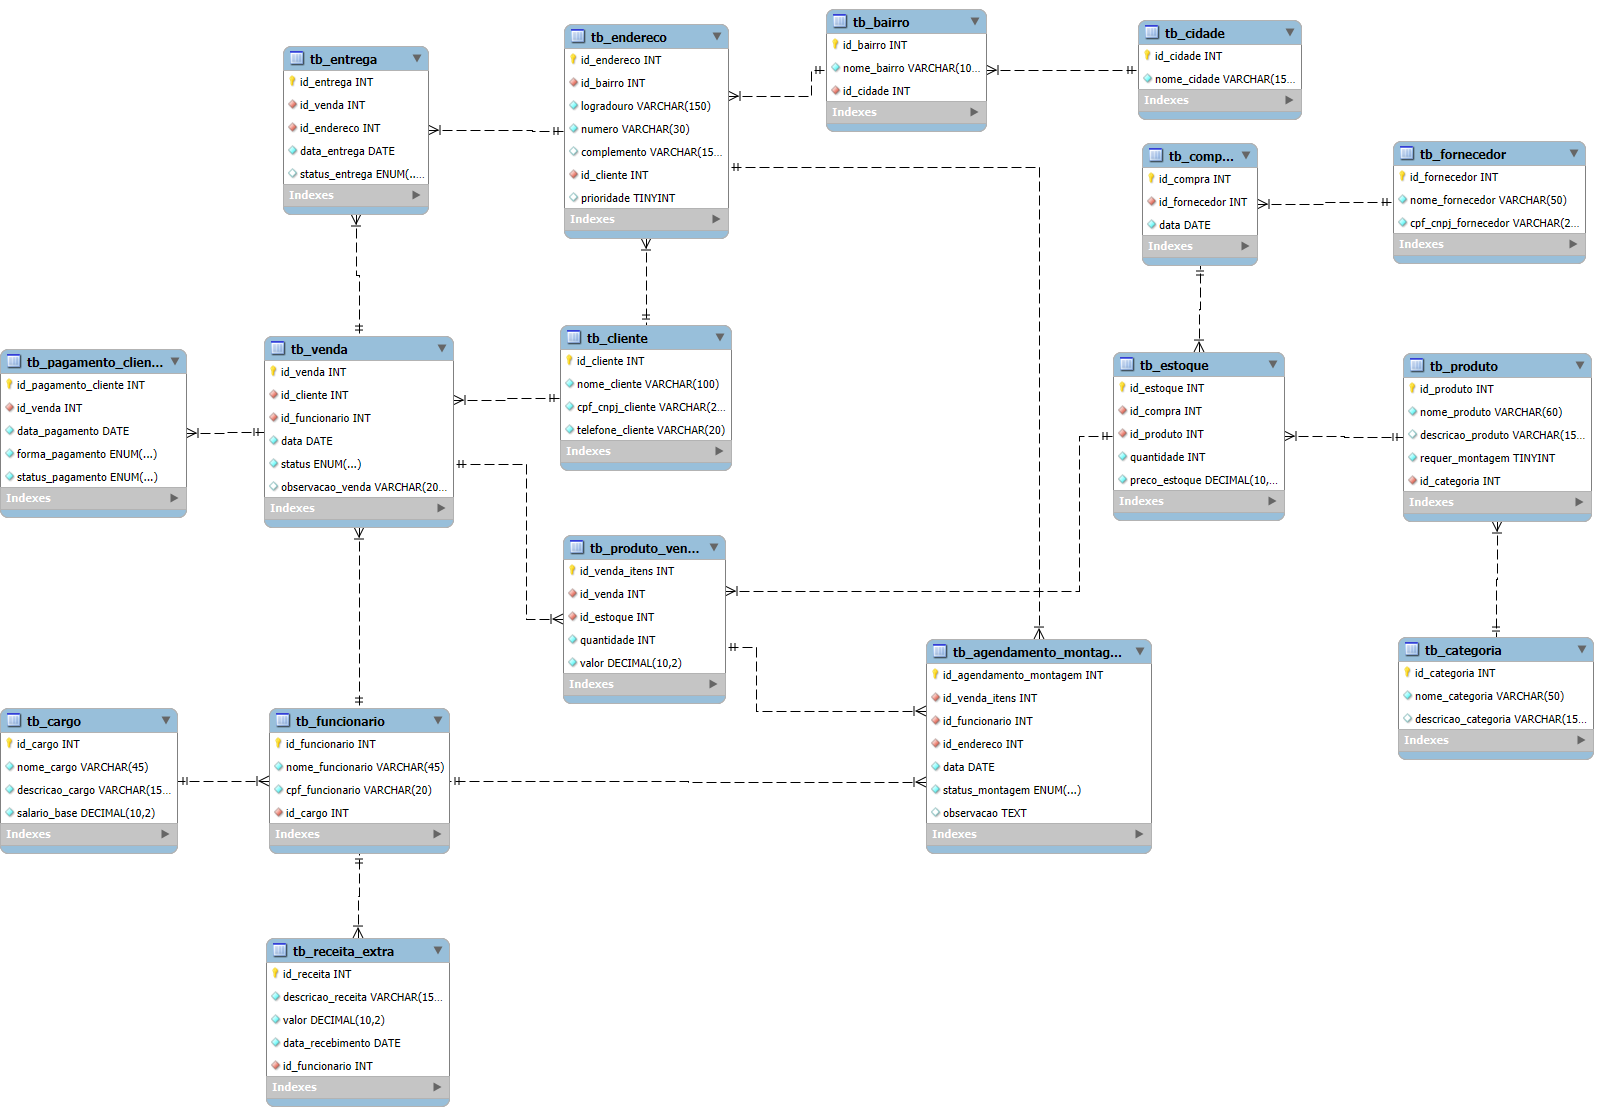
\includegraphics[width=.9\textwidth]{figuras/01-bdConceitualLog/mer.png}
    % %   \caption{Diagrama Modelo-Entidade}
    % %   \label{fig:mer}
    % % \end{figure}

    \section{Estrutura do Trabalho}\label{sec:EstruturaTrabalho}
    Após a definição conceitual/lógica, o banco deve ser implementado fisicamente em MySQL.
    Essa implementação, juntamente com a primeira carga de dados, é descrita no Capítulo~\ref{chap:fisico}.
    
    Com o banco implementado fisicamente, consultas nos dados podem ser realizadas por meio de \texttt{SQL}.
    O Capítulo apresenta inúmeras consultas, cada uma com uma característica diferente.
    
    Algumas rotinas podem ser definidas para automatizar tarefas e, em alguns casos, melhorar a performance:
    visões, funções, procedimentos, gatilhos e eventos. Esses recursos são tratados no Capítulo~\ref{chap:otimizacao}.
    
    O acesso aos dados deve ser controlado por segurança. Usuários distintos têm permissões distintas; isso é tratado no Capítulo~\ref{chap:acesso}.
    
    Para garantir propriedades ACID, operações de alteração devem ser realizadas em bloco de transação (Capítulo~\ref{chap:transacoes}).
    
    Por fim, falhas podem ocorrer; tolerâncias e tratamentos são descritos no Capítulo~\ref{chap:falhas}.
    
    \chapter{BANCO DE DADOS FÍSICO}\label{chap:fisico}
    A criação do ``\texttt{<nomeDoBD>}'' considerando MySQL é descrita na Seção~\ref{sec:def-fisica} por meio de DDL.
    A carga inicial é dada na Seção por meio de DML.
    
    \section{Definição Física}\label{sec:def-fisica}
    Os scripts responsáveis pela criação física do schema são descritos abaixo. Todas as restrições de integridade
    (chaves candidatas, primárias e estrangeiras) são consideradas no momento da criação.
    
    \begin{lstlisting}[language=SQL,caption={DDL -- Tabela \texttt{tb\_cliente}}]
    CREATE TABLE IF NOT EXISTS `mydb`.`tb_cliente` (
    `id_cliente` INT NOT NULL AUTO_INCREMENT,
    `nome_cliente` VARCHAR(100) NOT NULL,
    `cpf_cnpj_cliente` VARCHAR(20) NOT NULL,
    `telefone_cliente` VARCHAR(20) NOT NULL,
    PRIMARY KEY (`id_cliente`),
    UNIQUE INDEX `cpf_cnpj_cliente` (`cpf_cnpj_cliente` ASC) VISIBLE)
    \end{lstlisting}
    \begin{lstlisting}[language=SQL,caption={DDL -- Tabela \texttt{tb\_cargo}}]
    	CREATE TABLE IF NOT EXISTS `mydb`.`tb_cargo` (
    	`id_cargo` INT NOT NULL AUTO_INCREMENT,
    	`nome_cargo` VARCHAR(45) NOT NULL,
    	`descricao_cargo` VARCHAR(150) NOT NULL,
    	`salario_base` DECIMAL(10,2) NOT NULL,
    	PRIMARY KEY (`id_cargo`))
    \end{lstlisting}
    \begin{lstlisting}[language=SQL,caption={DDL -- Tabela \texttt{tb\_funcionario}}]
    	CREATE TABLE IF NOT EXISTS `mydb`.`tb_funcionario` (
    	`id_funcionario` INT NOT NULL AUTO_INCREMENT,
    	`nome_funcionario` VARCHAR(45) NOT NULL,
    	`cpf_funcionario` VARCHAR(20) NOT NULL,
    	`id_cargo` INT NOT NULL,
    	PRIMARY KEY (`id_funcionario`),
    	UNIQUE INDEX `cpf_funcionario` (`cpf_funcionario` ASC) VISIBLE,
    	INDEX `id_cargo` (`id_cargo` ASC) VISIBLE,
    	CONSTRAINT `tb_funcionario_ibfk_1`
    	FOREIGN KEY (`id_cargo`)
    	REFERENCES `mydb`.`tb_cargo` (`id_cargo`))KEY (sex_codigo)
    	);
    \end{lstlisting}
    \begin{lstlisting}[language=SQL,caption={DDL -- Tabela \texttt{tb\_venda}}]
    	CREATE TABLE IF NOT EXISTS `mydb`.`tb_venda` (
    	`id_venda` INT NOT NULL AUTO_INCREMENT,
    	`id_cliente` INT NOT NULL,
    	`id_funcionario` INT NOT NULL,
    	`data` DATE NOT NULL,
    	`status` ENUM('pendente', 'concluida', 'cancelada') NOT NULL,
    	`observacao_venda` VARCHAR(200) NULL DEFAULT NULL,
    	PRIMARY KEY (`id_venda`),
    	INDEX `id_cliente` (`id_cliente` ASC) VISIBLE,
    	INDEX `id_funcionario` (`id_funcionario` ASC) VISIBLE,
    	CONSTRAINT `tb_venda_ibfk_1`
    	FOREIGN KEY (`id_cliente`)
    	REFERENCES `mydb`.`tb_cliente` (`id_cliente`),
    	CONSTRAINT `tb_venda_ibfk_2`
    	FOREIGN KEY (`id_funcionario`)
    	REFERENCES `mydb`.`tb_funcionario` (`id_funcionario`))
    \end{lstlisting}
    \begin{lstlisting}[language=SQL,caption={DDL -- Tabela \texttt{tb\_cidade}}]
    	CREATE TABLE IF NOT EXISTS `mydb`.`tb_cidade` (
    	`id_cidade` INT NOT NULL AUTO_INCREMENT,
    	`nome_cidade` VARCHAR(150) NOT NULL,
    	PRIMARY KEY (`id_cidade`))
    \end{lstlisting}
    \begin{lstlisting}[language=SQL,caption={DDL -- Tabela \texttt{tb\_bairro}}]
    	CREATE TABLE IF NOT EXISTS `mydb`.`tb_bairro` (
    	`id_bairro` INT NOT NULL AUTO_INCREMENT,
    	`nome_bairro` VARCHAR(100) NOT NULL,
    	`id_cidade` INT NOT NULL,
    	PRIMARY KEY (`id_bairro`),
    	INDEX `id_cidade` (`id_cidade` ASC) VISIBLE,
    	CONSTRAINT `tb_bairro_ibfk_1`
    	FOREIGN KEY (`id_cidade`)
    	REFERENCES `mydb`.`tb_cidade` (`id_cidade`))
    \end{lstlisting}
    \begin{lstlisting}[language=SQL,caption={DDL -- Tabela \texttt{tb\_endereco}}]
    	CREATE TABLE IF NOT EXISTS `mydb`.`tb_endereco` (
    	`id_endereco` INT NOT NULL AUTO_INCREMENT,
    	`id_bairro` INT NOT NULL,
    	`rua` VARCHAR(150) NOT NULL,
    	`numero` VARCHAR(30) NOT NULL,
    	`complemento` VARCHAR(150) NULL DEFAULT NULL,
    	`id_cliente` INT NOT NULL,
    	`prioridade` TINYINT NULL DEFAULT NULL,
    	PRIMARY KEY (`id_endereco`),
    	INDEX `id_cliente` (`id_cliente` ASC) VISIBLE,
    	INDEX `id_bairro` (`id_bairro` ASC) VISIBLE,
    	CONSTRAINT `tb_endereco_ibfk_1`
    	FOREIGN KEY (`id_cliente`)
    	REFERENCES `mydb`.`tb_cliente` (`id_cliente`),
    	CONSTRAINT `tb_endereco_ibfk_2`
    	FOREIGN KEY (`id_bairro`)
    	REFERENCES `mydb`.`tb_bairro` (`id_bairro`))
    \end{lstlisting}
    \begin{lstlisting}[language=SQL,caption={DDL -- Tabela \texttt{tb\_agendamento\_montagem}}]
    	CREATE TABLE IF NOT EXISTS `mydb`.`tb_agendamento_montagem` (
    	`id_agendamento_montagem` INT NOT NULL AUTO_INCREMENT,
    	`id_venda` INT NOT NULL,
    	`id_funcionario` INT NOT NULL,
    	`id_endereco` INT NOT NULL,
    	`data` DATE NOT NULL,
    	`status_montagem` ENUM('realizado', 'pendente', 'cancelado') NOT NULL,
    	`observacao` TEXT NULL DEFAULT NULL,
    	PRIMARY KEY (`id_agendamento_montagem`),
    	INDEX `id_venda` (`id_venda` ASC) VISIBLE,
    	INDEX `id_funcionario` (`id_funcionario` ASC) VISIBLE,
    	INDEX `id_endereco` (`id_endereco` ASC) VISIBLE,
    	CONSTRAINT `tb_agendamento_montagem_ibfk_1`
    	FOREIGN KEY (`id_venda`)
    	REFERENCES `mydb`.`tb_venda` (`id_venda`),
    	CONSTRAINT `tb_agendamento_montagem_ibfk_2`
    	FOREIGN KEY (`id_funcionario`)
    	REFERENCES `mydb`.`tb_funcionario` (`id_funcionario`),
    	CONSTRAINT `tb_agendamento_montagem_ibfk_3`
    	FOREIGN KEY (`id_endereco`)
    	REFERENCES `mydb`.`tb_endereco` (`id_endereco`));
    \end{lstlisting}
    \begin{lstlisting}[language=SQL,caption={DDL -- Tabela \texttt{tb\_categoria}}]
	    CREATE TABLE IF NOT EXISTS `mydb`.`tb_categoria` (
	    `id_categoria` INT NOT NULL AUTO_INCREMENT,
	    `nome_categoria` VARCHAR(50) NOT NULL,
	    `descricao_categoria` VARCHAR(150) NULL DEFAULT NULL,
	    PRIMARY KEY (`id_categoria`),
	    UNIQUE INDEX `nome_categoria` (`nome_categoria` ASC); VISIBLE)
    \end{lstlisting}
    \begin{lstlisting}[language=SQL,caption={DDL -- Tabela \texttt{tb\_fornecedor}}]
    	CREATE TABLE IF NOT EXISTS `mydb`.`tb_fornecedor` (
    	`id_fornecedor` INT NOT NULL AUTO_INCREMENT,
    	`nome_fornecedor` VARCHAR(50) NOT NULL,
    	`cpf_cnpj_fornecedor` VARCHAR(20) NOT NULL,
    	PRIMARY KEY (`id_fornecedor`),
    	UNIQUE INDEX `cpf_cnpj_fornecedor` (`cpf_cnpj_fornecedor` ASC) VISIBLE)
    \end{lstlisting}
    \begin{lstlisting}[language=SQL,caption={DDL -- Tabela \texttt{tb\_compra}}]
    	CREATE TABLE IF NOT EXISTS `mydb`.`tb_compra` (
    	`id_compra` INT NOT NULL AUTO_INCREMENT,
    	`id_fornecedor` INT NOT NULL,
    	`data` DATE NOT NULL,
    	PRIMARY KEY (`id_compra`),
    	INDEX `id_fornecedor` (`id_fornecedor` ASC) VISIBLE,
    	CONSTRAINT `tb_compra_ibfk_1`
    	FOREIGN KEY (`id_fornecedor`)
    	REFERENCES `mydb`.`tb_fornecedor` (`id_fornecedor`))
    \end{lstlisting}
    \begin{lstlisting}[language=SQL,caption={DDL -- Tabela \texttt{tb\_entrega}}]
    	CREATE TABLE IF NOT EXISTS `mydb`.`tb_entrega` (
    	`id_entrega` INT NOT NULL AUTO_INCREMENT,
    	`id_venda` INT NOT NULL,
    	`id_endereco` INT NOT NULL,
    	`data_entrega` DATE NOT NULL,
    	`status_entrega` ENUM('pendente', 'entregue', 'cancelado') NULL DEFAULT 'pendente',
    	PRIMARY KEY (`id_entrega`),
    	INDEX `id_venda` (`id_venda` ASC) VISIBLE,
    	INDEX `id_endereco` (`id_endereco` ASC) VISIBLE,
    	CONSTRAINT `tb_entrega_ibfk_1`
    	FOREIGN KEY (`id_venda`)
    	REFERENCES `mydb`.`tb_venda` (`id_venda`),
    	CONSTRAINT `tb_entrega_ibfk_2`
    	FOREIGN KEY (`id_endereco`)
    	REFERENCES `mydb`.`tb_endereco` (`id_endereco`))
    \end{lstlisting}
    \begin{lstlisting}[language=SQL,caption={DDL -- Tabela \texttt{tb\_produto}}]
    	CREATE TABLE IF NOT EXISTS `mydb`.`tb_produto` (
    	`id_produto` INT NOT NULL AUTO_INCREMENT,
    	`nome_produto` VARCHAR(60) NOT NULL,
    	`descricao_produto` VARCHAR(150) NULL DEFAULT NULL,
    	`id_categoria` INT NOT NULL,
    	`id_fornecedor` INT NOT NULL,
    	PRIMARY KEY (`id_produto`),
    	UNIQUE INDEX `nome_produto` (`nome_produto` ASC) VISIBLE,
    	INDEX `id_categoria` (`id_categoria` ASC) VISIBLE,
    	INDEX `id_fornecedor` (`id_fornecedor` ASC) VISIBLE,
    	CONSTRAINT `tb_produto_ibfk_1`
    	FOREIGN KEY (`id_categoria`)
    	REFERENCES `mydb`.`tb_categoria` (`id_categoria`),
    	CONSTRAINT `tb_produto_ibfk_2`
    	FOREIGN KEY (`id_fornecedor`)
    	REFERENCES `mydb`.`tb_fornecedor` (`id_fornecedor`))
    \end{lstlisting}
    \begin{lstlisting}[language=SQL,caption={DDL -- Tabela \texttt{tb\_estoque}}]
    	CREATE TABLE IF NOT EXISTS `mydb`.`tb_estoque` (
    	`id_estoque` INT NOT NULL AUTO_INCREMENT,
    	`id_compra` INT NOT NULL,
    	`id_produto` INT NOT NULL,
    	`quantidade` INT NOT NULL,
    	`preco_estoque` DECIMAL(10,2) NOT NULL,
    	PRIMARY KEY (`id_estoque`),
    	INDEX `id_compra` (`id_compra` ASC) VISIBLE,
    	INDEX `id_produto` (`id_produto` ASC) VISIBLE,
    	CONSTRAINT `tb_estoque_ibfk_1`
    	FOREIGN KEY (`id_compra`)
    	REFERENCES `mydb`.`tb_compra` (`id_compra`),
    	CONSTRAINT `tb_estoque_ibfk_2`
    	FOREIGN KEY (`id_produto`)
    	REFERENCES `mydb`.`tb_produto` (`id_produto`))
    \end{lstlisting}
    \begin{lstlisting}[language=SQL,caption={DDL -- Tabela \texttt{tb\_pagamento\_cliente}}]
    	CREATE TABLE IF NOT EXISTS `mydb`.`tb_pagamento_cliente` (
    	`id_pagamento_cliente` INT NOT NULL AUTO_INCREMENT,
    	`id_venda` INT NOT NULL,
    	`data_pagamento` DATE NOT NULL,
    	`forma_pagamento` ENUM('cartao_credito', 'cartao_debito', 'pix', 'boleto', 'dinheiro') NOT NULL,
    	`status_pagamento` ENUM('pendente', 'pago', 'cancelado', 'atrasado') NOT NULL,
    	PRIMARY KEY (`id_pagamento_cliente`),
    	INDEX `id_venda` (`id_venda` ASC) VISIBLE,
    	CONSTRAINT `tb_pagamento_cliente_ibfk_1`
    	FOREIGN KEY (`id_venda`)
    	REFERENCES `mydb`.`tb_venda` (`id_venda`))
    \end{lstlisting}
    \begin{lstlisting}[language=SQL,caption={DDL -- Tabela \texttt{tb\_sexo}}]
    	CREATE TABLE tb_sexo (
    	sex_codigo   INT          NOT NULL AUTO_INCREMENT,
    	sex_descricao VARCHAR(45) NOT NULL UNIQUE,
    	PRIMARY KEY (sex_codigo)
    	);
    \end{lstlisting}
    \begin{lstlisting}[language=SQL,caption={DDL -- Tabela \texttt{tb\_produto\_venda}}]
    	CREATE TABLE IF NOT EXISTS `mydb`.`tb_produto_venda` (
    	`id_venda_itens` INT NOT NULL AUTO_INCREMENT,
    	`id_venda` INT NOT NULL,
    	`id_produto` INT NOT NULL,
    	`quantidade` INT NOT NULL,
    	`valor` DECIMAL(10,2) NOT NULL,
    	PRIMARY KEY (`id_venda_itens`),
    	INDEX `id_venda` (`id_venda` ASC) VISIBLE,
    	INDEX `id_produto` (`id_produto` ASC) VISIBLE,
    	CONSTRAINT `tb_produto_venda_ibfk_1`
    	FOREIGN KEY (`id_venda`)
    	REFERENCES `mydb`.`tb_venda` (`id_venda`),
    	CONSTRAINT `tb_produto_venda_ibfk_2`
    	FOREIGN KEY (`id_produto`)
    	REFERENCES `mydb`.`tb_produto` (`id_produto`))
    \end{lstlisting}
    \begin{lstlisting}[language=SQL,caption={DDL -- Tabela \texttt{tb\_receita\_extra}}]
    	CREATE TABLE IF NOT EXISTS `mydb`.`tb_receita_extra` (
    	`id_receita` INT NOT NULL AUTO_INCREMENT,
    	`descricao_receita` VARCHAR(150) NOT NULL,
    	`valor` DECIMAL(10,2) NOT NULL,
    	`data_recebimento` DATE NOT NULL,
    	`id_funcionario` INT NOT NULL,
    	PRIMARY KEY (`id_receita`),
    	INDEX `id_funcionario` (`id_funcionario` ASC) VISIBLE,
    	CONSTRAINT `tb_receita_extra_ibfk_1`
    	FOREIGN KEY (`id_funcionario`)
    	REFERENCES `mydb`.`tb_funcionario` (`id_funcionario`))
    \end{lstlisting}

    \section{Carga de Dados Iniciais}\label{sec:carga}
    Após a criação do banco, uma carga inicial é inserida por meio de DML:
    
    \begin{lstlisting}[language=SQL,caption={DML -- Tabela \texttt{tb\_cargo}}]
        INSERT INTO tb_cargo (nome_cargo, descricao_cargo, salario_base) VALUES
        ('Vendedor','Responsável pelo atendimento e vendas em loja',2000.00),
        ('Montador','Realiza montagem de móveis',2200.00),
        ('Gerente','Gerencia a equipe e as metas da loja',4500.00);
    \end{lstlisting}
    \begin{lstlisting}[language=SQL,caption={DML -- Tabela \texttt{tb\_funcionario}}]
    INSERT INTO tb_funcionario (nome_funcionario, cpf_funcionario, id_cargo) VALUES
    ('José Seben','00000000000',3),
    ('Caio Macedo','11111111111',1),
    ('Kaique Lima','22222222222',2),
    ('Fernando Buligon','33333333333',1);
    \end{lstlisting}
    
    \begin{lstlisting}[language=SQL,caption={DML -- Tabela \texttt{tb\_cliente}}]
        INSERT INTO tb_cliente (nome_cliente, cpf_cnpj_cliente, telefone_cliente) VALUES
        ('João Oliveira','00000000000','(00) 00000-0000'),
        ('Maria Santos','11111111111','(11) 11111-1111'),
        ('Eduardo Costa','22222222222','(22) 22222-2222'),
        ('Gabriela Barros','33333333333','(33) 33333-3333'),
        ('Pedro Cachoeira','44444444444','(44) 44444-4444');
    \end{lstlisting}
    
    \begin{lstlisting}[language=SQL,caption={DML -- Tabela \texttt{tb\_cidade}}]
        INSERT INTO tb_cidade (nome_cidade) VALUES
        ('Santa Helena'),
        ('Sao Clemente'),
        ('Medianeira'),
        ('Subsede'),
        ('Entre Rios');
    \end{lstlisting}
    
    \begin{lstlisting}[language=SQL,caption={DML -- Tabela \texttt{tb\_bairro}}]
        INSERT INTO tb_bairro (nome_bairro, id_cidade) VALUES
        ('Centro',1),
        ('Centro',2),
        ('Centro',3),
        ('Centro',4),
        ('Centro',5);
    \end{lstlisting}
    
    \begin{lstlisting}[language=SQL,caption={DML -- Tabela \texttt{tb\_endereco}}]
        INSERT INTO tb_endereco (id_bairro, rua, numero, complemento, id_cliente, prioridade) VALUES
        (1,'Rua Xaxim','123',NULL,1,1),
        (2,'Av. Brasil','321',NULL,2,1),
        (3,'Rua Aroeira','231',NULL,3,1),
        (4,'Rua Argentina','213',NULL,4,1),
        (4,'Rua Argentina','312',NULL,5,1);
    \end{lstlisting}
    
    \begin{lstlisting}[language=SQL,caption={DML -- Tabela \texttt{tb\_categoria}}]
        INSERT INTO tb_categoria (nome_categoria, descricao_categoria) VALUES
        ('Ferramentas','Makita, martelo, pá...'),
        ('Mobilia','Guarda-roupa, mesa, bancada...'),
        ('Materiais','Areia, pedra, prego...');
    \end{lstlisting}
    
    \begin{lstlisting}[language=SQL,caption={DML -- Tabela \texttt{tb\_fornecedor}}]
        INSERT INTO tb_fornecedor (nome_fornecedor, cpf_cnpj_fornecedor) VALUES
        ('Kaique Madeiras','22222222222222'),
        ('João das Areias','33333333333333'),
        ('Pedro Pedradas','44444444444444'),
        ('Rafael Pregos','55555555555555'),
        ('Raul Rolamentos','66666666666666');
    \end{lstlisting}
    
    \begin{lstlisting}[language=SQL,caption={DML -- Tabela \texttt{tb\_produto}}]
        INSERT INTO tb_produto (nome_produto, descricao_produto, id_categoria, id_fornecedor) VALUES
        ('Makita 5007N','Serra Circular 7-1/4 1800W',1,1),
        ('Madeira Pinus','Madeira boa',3,1),
        ('Mesa Retangular','Mesa de madeira',2,1),
        ('Pedra Brita','Essa é da boa',3,3),
        ('Areia Média','Funciona bem',3,2);
    \end{lstlisting}
    
    \begin{lstlisting}[language=SQL,caption={DML -- Tabela \texttt{tb\_compra}}]
        INSERT INTO tb_compra (id_fornecedor, data) VALUES
        (1,'2025-08-10'),
        (1,'2025-08-11'),
        (1,'2025-08-12'),
        (1,'2025-08-13');
    \end{lstlisting}
    
    \begin{lstlisting}[language=SQL,caption={DML -- Tabela \texttt{tb\_estoque}}]
        INSERT INTO tb_estoque (id_compra, id_produto, quantidade, preco_estoque) VALUES
        (1,1, 50, 793.78),
        (2,2,100, 120.00),
        (2,3, 20, 450.00),
        (3,4,200,  35.00),
        (4,5,180,  30.00);
    \end{lstlisting}
    
    \begin{lstlisting}[language=SQL,caption={DML -- Tabela \texttt{tb\_venda}}]
        INSERT INTO tb_venda (id_cliente, id_funcionario, data, status, observacao_venda) VALUES
        (1,2,'2025-08-15','concluida','Cara saiu feliz'),
        (2,2,'2025-08-16','pendente','Aguardando pagamento'),
        (3,4,'2025-08-17','concluida','Sucesso'),
        (4,4,'2025-08-18','cancelada','Cartão não passou');
    \end{lstlisting}
    
    \begin{lstlisting}[language=SQL,caption={DML -- Tabela \texttt{tb\_produto\_venda}}]
        INSERT INTO tb_produto_venda (id_venda, id_produto, quantidade, valor) VALUES
        (1,1,189,793.78),
        (2,1,  1,793.78),
        (3,1,  1,793.78),
        (4,1,  1,793.78);
    \end{lstlisting}
    
    \begin{lstlisting}[language=SQL,caption={DML -- Tabela \texttt{tb\_pagamento\_cliente}}]
        INSERT INTO tb_pagamento_cliente (id_venda, data_pagamento, forma_pagamento, status_pagamento) VALUES
        (1,'2025-08-15','pix','pago'),
        (2,'2025-08-17','boleto','pendente'),
        (3,'2025-08-17','boleto','pago'),
        (4,'2025-08-18','cartao\_credito','cancelado');
    \end{lstlisting}
    
    \begin{lstlisting}[language=SQL,caption={DML -- Tabela \texttt{tb\_entrega}}]
        INSERT INTO tb_entrega (id_venda, id_endereco, data_entrega, status_entrega) VALUES
        (1,1,'2025-08-16','entregue'),
        (2,2,'2025-08-20','pendente'),
        (3,3,'2025-08-18','entregue');
    \end{lstlisting}
    
    \begin{lstlisting}[language=SQL,caption={DML -- Tabela \texttt{tb\_agendamento\_montagem}}]
        INSERT INTO tb_agendamento_montagem (id_venda, id_funcionario, id_endereco, data, status_montagem, observacao) VALUES
        (1,2,1,'2025-08-16','realizado','Cliente chato'),
        (2,2,2,'2025-08-21','pendente','No aguardo da chegada dos materiais'),
        (3,2,3,'2025-08-19','realizado','Sucesso');
    \end{lstlisting}
    
    \begin{lstlisting}[language=SQL,caption={DML -- Tabela \texttt{tb\_receita\_extra}}]
        INSERT INTO tb_receita_extra (descricao_receita, valor, data_recebimento, id_funcionario) VALUES
        ('Rapaz merece',350.00,'2025-08-19',2),
        ('Bateu o recorde em montagem de balcão',120.00,'2025-08-19',3),
        ('Comprou makita',150.00,'2025-08-20',1);
    \end{lstlisting}


\chapter{CONSULTAS DE DADOS NO BD}\label{chap:consultas}
A linguagem SQL permite diferentes recursos para recuperar informações.
As seções abaixo listam os tipos de consultas (exemplos a completar).
    
    \section{Restrições de Linha}
    
    \begin{lstlisting}[language=SQL,caption={SELECT -- Tabela\texttt{tb\_cliente}}]
        SELECT * FROM tb_cliente
        WHERE cpf_cnpj_cliente IN ('00000000000','11111111111');
    \end{lstlisting}
    
    \begin{lstlisting}[language=SQL,caption={SELECT -- Tabela \texttt{tb\_cargo}}]
        SELECT * FROM tb_cargo
        WHERE salario_base > 3000.00;
    \end{lstlisting}
    
    \begin{lstlisting}[language=SQL,caption={SELECT -- Tabela \texttt{tb\_funcionario}}]
        SELECT * FROM tb_funcionario
        WHERE id_cargo = 1;
    \end{lstlisting}
    
    \begin{lstlisting}[language=SQL,caption={SELECT -- Tabela \texttt{tb\_venda}}]
        SELECT * FROM tb_venda
        WHERE status = 'concluida'
    \end{lstlisting}
    
    \begin{lstlisting}[language=SQL,caption={SELECT -- Tabela \texttt{tb\_cidade}}]
        SELECT * FROM tb_cidade
        WHERE nome_cidade IN ('Santa Helena','Medianeira');
    \end{lstlisting}
    
    \begin{lstlisting}[language=SQL,caption={SELECT -- Tabela \texttt{tb\_bairro}}]
        SELECT * FROM tb_bairro
        WHERE nome_bairro = 'Centro'
        AND id_cidade IN (4,5);
    \end{lstlisting}
    
    \begin{lstlisting}[language=SQL,caption={SELECT -- Tabela \texttt{tb\_endereco}}]
        SELECT * FROM tb_endereco
        WHERE id_cliente IN (1,5)
        AND complemento IS NULL;
    \end{lstlisting}
    
    \begin{lstlisting}[language=SQL,caption={SELECT -- Tabela \texttt{tb\_agendamento\_montagem}}]
        SELECT * FROM tb_agendamento_montagem
        WHERE status_montagem = 'realizado'
        AND data >= '2025-08-19';
    \end{lstlisting}
    
    \begin{lstlisting}[language=SQL,caption={SELECT -- Tabela \texttt{tb\_categoria}}]
        SELECT * FROM tb_categoria
        WHERE nome_categoria <> 'Ferramentas';
    \end{lstlisting}
    
    \begin{lstlisting}[language=SQL,caption={SELECT -- Tabela \texttt{tb\_fornecedor}}]
        SELECT * FROM tb_fornecedor
        WHERE cpf_cnpj_fornecedor LIKE '33%';
    \end{lstlisting}
    
    \begin{lstlisting}[language=SQL,caption={SELECT -- Tabela \texttt{tb\_compra}}]
        SELECT * FROM tb_compra
        WHERE id_fornecedor = 1
        AND data >= '2025-08-12';
    \end{lstlisting}
    
    \begin{lstlisting}[language=SQL,caption={SELECT -- Tabela \texttt{tb\_entrega}}]
        SELECT * FROM tb_entrega
        WHERE status_entrega = 'pendente'
        OR data_entrega > '2025-08-17';
    \end{lstlisting}
    
    \begin{lstlisting}[language=SQL,caption={SELECT -- Tabela \texttt{tb\_produto}}]
        SELECT * FROM tb_produto
        WHERE id_categoria = 3
        AND descricao_produto IS NOT NULL;
    \end{lstlisting}
    
    \begin{lstlisting}[language=SQL,caption={SELECT -- Tabela \texttt{tb\_estoque}}]
        SELECT * FROM tb_estoque
        WHERE quantidade >= 100
        AND preco_estoque <= 120.00;
    \end{lstlisting}
    
    \begin{lstlisting}[language=SQL,caption={SELECT -- Tabela \texttt{tb\_pagamento\_cliente}}]
        SELECT * FROM tb_pagamento_cliente
        WHERE forma_pagamento IN ('pix','boleto')
        AND status_pagamento = 'pago';
    \end{lstlisting}
    
    \begin{lstlisting}[language=SQL,caption={SELECT -- Tabela \texttt{tb\_produto\_venda}}]
        SELECT * FROM tb_produto_venda
        WHERE id_produto = 1
        AND quantidade >= 100;
    \end{lstlisting}
    
    \begin{lstlisting}[language=SQL,caption={SELECT -- Tabela \texttt{tb\_receita\_extra}}]
        SELECT * FROM tb_receita_extra
        WHERE data_recebimento BETWEEN '2025-08-19' AND '2025-08-20'
        AND valor >= 150.00;
    \end{lstlisting}
    
    \section{Funções de Linha}
    \dots
    
    \section{Junções de Tabelas}
    \dots
    
    \section{Operadores de Conjunto}
    \dots
    
    \section{Sub-Consultas}
    \dots
    
    \section{Agregação e Funções de Agrupamento}
    \dots
    
    \section{\texttt{SELECT} nos Comandos}
    \dots

\chapter{ROTINAS DE OTIMIZAÇÃO NO BD}\label{chap:otimizacao}
    \section{Visões}
    \dots
    
    \section{Funções}
    \dots
    
    \section{Procedimentos}
    \dots
    
    \section{Gatilhos}
    \dots
    
    \section{Eventos}
    \dots

\chapter{CONTROLE DE ACESSO}\label{chap:acesso}
O controle de acesso é dado por \texttt{GRANT} e \texttt{REVOKE}. As subseções a seguir seguem o PDF.
    
    \section{Criar Usuários}
    \dots
    
    \section{Atribuir Permissões}
    \dots
    
    \section{Revogar Permissões}
    \dots
    
\chapter{TRANSAÇÕES NO BD}\label{chap:transacoes}
Defina blocos transacionais atômicos para preservar ACID.
\dots

\chapter{FALHAS NO BD}\label{chap:falhas}
Durante a execução de qualquer software, falhas podem ocorrer; tolerâncias e tratamentos devem ser estabelecidos.

    \section{Tolerâncias à Falhas}
    \dots
    
    \section{Tratamento à Falhas}
    \dots

% --- Referências (livre; substitua por biblatex se quiser)
\clearpage
\chapter*{REFERÊNCIAS}
\addcontentsline{toc}{chapter}{REFERÊNCIAS}
% Insira suas referências manualmente ou troque para biblatex.
\vspace{-0.5em}
\begin{itemize}
  \item \dots
\end{itemize}

\end{document}
